\documentclass[prodmode,acmtoms]{acmsmall}
%  

% Package to generate and customize Algorithm as per ACM style
\usepackage[ruled]{algorithm2e}
\renewcommand{\algorithmcfname}{ALGORITHM}
\SetAlFnt{\small}
\SetAlCapFnt{\small}
\SetAlCapNameFnt{\small}
\SetAlCapHSkip{0pt}
\IncMargin{-\parindent}

% Metadata Information
\acmVolume{0}
\acmNumber{0} 
\acmArticle{00}
\acmYear{0000}
\acmMonth{0}
 
%
%%% User-requested packages placed after this line %%%%%%%%%%%%%%%%%%%%%%%%%%%%
\usepackage{amsfonts,amssymb,amsmath}
\usepackage{booktabs,dcolumn}
\usepackage[T1]{fontenc}
\usepackage{mathtools}
\usepackage{enumerate,graphicx}
\usepackage{subfig}
\usepackage{multirow}
\usepackage{listings}

% \usepackage[center]{subfigure}
\numberwithin{equation}{section}
\usepackage{braket}                             %Provides \Set for typing sets
\usepackage{float} 
\usepackage{subfig}


%%% User's macros placed after this line %%%%%%%%%%%%%%%%%%%%%%%%%%%%%%%%%%%%%%
%\IfFileExists{dsfont.sty}%
%\usepackage{dsfont}
\newcommand{\R}{\mathbb{R}}
\newcommand{\N}{\mathbb{N}}
\renewcommand{\phi}{\varphi}
\renewcommand{\epsilon}{\varepsilon}
\newcommand{\deal}{\texttt{deal.II}}
\newcommand{\dope}{\texttt{DOpElib}}
\newcommand{\re}{\operatorname{Re}}

\newcommand{\todo}[1]{\textbf{\textsc{\textcolor{black}{TODO: #1}}}}
%\newcommand{\mymarginpar}[1]{\marginpar{\textcolor{red}{\scriptsize{#1}}}}
\newcommand{\mymarginpar}[1]{\marginpar{\textcolor{red}{\normalsize{#1}}}}
%
\begin{document}
\markboth{C. Goll, T. Wick, and W. Wollner}{DOpElib:  A Goal Oriented Software Library}

\title{DOpElib: Differential Equations and Optimization Environment; A Goal Oriented Software Library for Solving PDEs and Optimization Problems}

\author{CHRISTIAN GOLL
\affil{University of Heidelberg}
THOMAS WICK
\affil{The University of Texas at Austin}
WINNIFRIED WOLLNER
\affil{University of Hamburg}}

%%%%%%%%%%%%%%%%%%%%%%%%%%%%%%%%%%%%%%%%%%%

\begin{abstract}
In this article, we describe the software library 
\textit{Differential Equations and Optimization Environment} (\dope{}).
The main feature of \dope{} is that it provides a unified interface to high level algorithms 
such as time-stepping methods, nonlinear solvers and optimization routines. This structure ensures 
that first of all the user is required to write only those sections of code that are specific to 
the considered problem. Second, the exchange of parts of the used routines is possible 
with only a few lines of code to change instead of large reimplementations.
The article illustrates the design principles and various features
of the \dope{} and provides some 
numerical results as demonstration for the versatility of the software.
\end{abstract}

\begin{bottomstuff}
Author's adresses: C. Goll, Institut f\"ur Angewandte Mathematik,
Universit\"at Heidelberg;
T. Wick, The Institute for Computational Engineering and Sciences;
W. Wollner, Fachbereich Mathematik, Universit\"at Hamburg.
\end{bottomstuff}
                      

\maketitle
%%%%%%%%%%%%%%%%%%%%%%%%%%%%%%%%%%%%%%%%%%%


%%%%%%%%%%%%%%%%%%%%%%%%%%%%%%%%%%%%%%%%%%%
\section{Introduction}
\label{introduction}
Today, there exist a broad variety of software libraries
that provide numerical tools for solving partial differential
equations (PDEs). Prominent examples are 
\deal{} \cite{dealnew}, dune \cite{dune}, 
FEniCS \cite{fenics}
or commercial solvers like ANSYS (with its Fluent package) \cite{ansys},
COMSOL \cite{comsol} or simufact forming \cite{simufact}.
Finally, often, a lot of work is (still) done in Matlab \cite{matlab}.
In fact, these libraries provide very useful tools 
for a huge variety of applications. 

However, often, the user is confronted with 
certain bottlenecks. On the one hand, 
in open-source projects for academic research, 
standard high-level routines 
which are necessary to solve even simplest PDEs,
such as linear and nonlinear solvers or time-stepping schemes must be implemented 
by the users themselves. However, such routines are, at large,
problem-independent and could be provided as standard tools. 
As our guiding design principle, we note that in many 
numerical studies, the main task is the computation of some  
target functional, e.g., error norms,
point values, or certain mean-values as drag or lift coefficients.
As a second motivating principle, 
there is nowadays an increasing interest in computing 
optimization problems in which the state equation is governed 
by a PDE. Such optimization problems comprise optimal control,
parameter estimation, inverse problems or optimal experimental design. 
To do this in complex applications usually requires tremendous work already
on the PDE itself before considering optimization of the processes modeled 
by the PDE. Thus it is advantageous to have an environment that allows to 
focus on the development of an appropriate code for the PDE at first but 
asserts due to the required interface, that the code written for the PDE
is then reusable for the application of state-of-the-art optimization 
routines.
So far, there exist a very limited number of open source packages
which fulfill the requirements listed above; 
sucessful in-house code examples are Gascoigne \cite{gascoigne}
and RoDoBo \cite{rodobo}. 
Both have been initiated as well in 
the Numerical Analysis Group in Heidelberg.

On the other hand, commercial finite element toolkits provide these 
previously mentioned routines but limits user-interaction
with the source code to an extend that typically conflicts
with the consideration of problems deviating from the intended 
user-base for the commercial product. 
This is quite unsatisfactory because development of novel numerical 
algorithms should enable the researcher
to change certain parameters or pieces of source code. 

The presented toolkit \dope{}: 
\textit{Differential Equations and Optimization Environment}
fills this gap. We present a software
to solve both PDE problems as well as optimization problems 
constrained by a PDE. 
Its main feature is to give a unified interface to high level algorithms such as 
time-stepping methods, nonlinear solvers and optimization routines. 
\dope{} is designed such that the user only needs to write those parts
of the code that are problem dependent while all invariant 
parts of the algorithms
are reusable without any need for further coding.
In particular, the user is enabled to switch between various different 
algorithms without the need to rewrite the problem dependent code, 
though obviously he or she will
have to replace the algorithm object with an other one. 
This replacement can be done by replacing the appropriate object at only
one point in the code.

While \deal{} --which at present is the only toolkit to which we provide an 
interface-- leaves the implementation of all high-level algorithms to the user, 
\dope{} is user-focused by delivering
prefabricated tools which require from the user only adjustments connected
to his specific problem. The solution of optimization problems with PDE
constraints is an innovative feature in \dope{}.

The project was initially initiated at the University of Heidelberg in 2010 and  
at the present stage the following key features are supported by the library
\begin{itemize}
\item Solution of nonlinear stationary and nonstationary PDEs in 1d, 2d, and 3d.
\item Various, easily exchangeable, 
  time-stepping schemes (based on finite differences), 
  such as forward Euler, backward Euler,
  Crank-Nicolson, shifted Crank-Nicolson, and Fractional-Step-$\Theta$ scheme.
\item Use of all finite elements of from \deal{} including hp-support.
\item Several examples showing the solution of several PDEs including
   Poisson, Navier-Stokes, Plasticity and fluid-structure interaction problems. 
\item Line search and trust region newton algorithms for the 
   solution of optimization problems with PDEs by elimination of 
   the state variable. \cite{NoWr00} 
   \marginpar{spaeter zitieren}
\item Interface to SNOPT for the solution of optimization problems with PDEs and
  additional other control and state constraints.
\item Several examples showing how to solve various kinds of optimization 
  problems involving PDE constraints.
\item Goal-oriented mesh adaptation with the Dual Weighted Residual method, 
  following \cite{BR03}.
\item Different spatial triangulations for control and state variables without
  the need to reimplement the user dependent code when switching from one common 
  triangulation to different ones.
\end{itemize}

The article is organized as follows. In the main Section
\ref{detailed_description}, a detailed description of 
the main features is given. In fact, we first explain the solution 
of stationary PDEs, nonstationary PDEs, and optimization problems. 
Additional comments are given concerning the required implementation 
provided by the user.
Finally, additional features are discussed. In the final Section
\ref{applications}, we discuss three different numerical 
examples which illustrate the versatile features of \dope{}. 



%%%%%%%%%%%%%%%%%%%%%%%%%%%%%%%%%%%%%%%%%%%
\section{Detailed Description of the Main Features}
\label{detailed_description}
This library is designed to allow easy implementation and numerical solutions 
of problems involving partial differential equations (PDEs). 
In particular, we remove all tedious routine implementation needed in 
\deal{} by introducing appropriate classes that take care of all the 
problem independent implementation while leaving only the problem specific 
part to the user. To show how this is designed we will, in the sequel, 
describe the reasoning first for a simple stationary PDE in 
Section~\ref{subsubsec:stationary problems} and then show
how this idea extends to non stationary problems in 
Section~\ref{sec:timedep} as well as to optimization
problems with PDE constraints in Section~\ref{sec:opt}. 

\subsection{Solving of Stationary PDEs}
\label{subsubsec:stationary problems}
For the start we consider a prototypical problem given by the solution of 
a stationary PDE, which we assume to be given in weak form.
In abstract notation it reads; find some $u$ in an appropriate set
such that
\begin{align}\label{eq:prototype_weak}
a(u)(\phi) = (f,\phi) \quad \forall \phi \in V,
\end{align}
with some suitable space $V$ for the test functions and a 
right hand side function $f$.
To illustrate this further, we take the stationary 
incompressible Navier-Stokes equations in a domain $\Omega \subset \R^d$, 
i.e., $u = (v,p)$ and $\phi = (\phi_u,\phi_p)$ then
\begin{align}\label{eq:ns}
a(u)(\phi) = \nu(\nabla v, \nabla\phi_u) + (v \nabla v,\phi_u) + (p, \nabla \cdot \phi_u) + (\nabla \cdot v ,\phi_p)
\end{align}
for all $\phi \in V = H^1_0(\Omega;\R^d) \times L^2_0(\Omega)$.
Here $(\cdot,\cdot)$ denotes the $L^2$-inner-product.
The solution will be searched for in $V + (u_d,0)$ where $u_d$ is some 
continuation of the given Dirichlet boundary data.
Then typically we do not only want to calculate $u$ but more likely we are 
interested in one (or several) functionals depending on the solution, i.e., some numbers $J(u)$.

In order to solve this problem, i.e., calculate $J(u)$, we need to discretize 
the equation. In \dope, we are using finite elements to do this. This means we need to pick a 
subdivision $\mathcal T_h$, for instance into quadrilaterals,
of the domain $\Omega$ and a finite element. In the concrete case, we could, 
for instance, take the $\mathcal Q_2/\mathcal Q_1$ Taylor-Hood element.
As it is clear, that the initialization of the unknowns, the local shape 
functions, removal of hanging node constraints, etc. always follows the 
same procedure, we define an object which takes the finite element (FE)
and the triangulation and takes care of all other things related to
handling the finite element space $V_h$. We will refer, to 
this as the \texttt{SpaceTimeHandler}. Then, it is clear that the simplest 
form of the constructor should have the following interface:
\begin{lstlisting}
  template<typename Triangulation, typename FE>
      void SpaceTimeHandler(Triangulation &, FE);
\end{lstlisting}
Next, one needs to solve the discrete equation
\begin{align}\label{eq:discrete_equation}
a(u_h)(\phi_h) = (f,\phi_h) \quad \forall \phi \in V_h.
\end{align}
To this end, one can employ a newton type method with some globalization 
like line-search. To do so, one needs to calculate the residual of the 
equation, as well as to solve linearized equations for the calculation of 
the newton method and then employing some kind of globalization strategy.
This again will usually require the evaluation of the residual.

The evaluation of the residual will require the calculation of the integrals 
involved in the weak formulation of the problem. For example 
the $i$-th component of the residual, with respect to the given FE-basis 
$\phi_{h}^{i}$, will read as follows
\begin{align}\label{eq:residual_vector}
 a(u_h)(\phi_{h}^{i}) - (f,\phi_{h}^{i}) = \sum_{K\in \mathcal T_h} \nu\int_K \nabla u_h\cdot \nabla \phi_{h}^{i}\,dx + \ldots
 \end{align}
Again, we see that, except for the local element integrals, all 
calculations are independent from the concrete form of the PDE. 
Hence we define an object \texttt{Integrator}
that offers a method to calculate the residual given a user-defined 
object \texttt{pde} that implements the local element integrals, i.e.,
\begin{lstlisting}
  template<typename PROBLEM,typename VECTOR>
      void Integrator
             ::ComputeNonlinearResidual(PROBLEM& pde, 
                                        VECTOR & residual);
\end{lstlisting}
where \texttt{VECTOR} is one of the possible vector types given by \deal{}.
It is clear that we need to ensure that the integrator object has access
to the information stored in the \texttt{SpaceTimeHandler}
to correctly loop over all elements.
To solve the linearized systems, again, all that is left is the calculation
of the matrix corresponding to the linearized equation. To calculate this,
 we can define a method in the integrator that does exactly this provided
we have a user defined object \texttt{pde} that can evaluate the local 
integrals needed for assembling the matrix, i.e.,
\begin{lstlisting}
  template<typename PROBLEM,typename MATRIX>
      void Integrator
             ::ComputeMatrix(PROBLEM& pde, 
                             MATRIX & system_matrix);
\end{lstlisting}
where now \texttt{MATRIX} is one of the matrix types supported by \deal{}.
With this we can now define a nonlinear solver \texttt{NewtonSolver} 
for the solution of the discrete problem requiring the existence of the 
following function
\begin{lstlisting}
 template<typename LINSOLVE>
  template<typename PROBLEM, typename VECTOR>
      void NewtonSolver<LINSOLVE>
             ::NonlinearSolve(PROBLEM& pde, 
                              VECTOR & solution);
\end{lstlisting}
Where \texttt{LINSOLVE} denotes the solver that should be used to solve the 
linearized equations during the newton iteration.

Finally, we note that to compute the requested functional value 
all that is left is to evaluate the functional in the computed solution 
which can be done again using an appropriate integrator method.
Since the sequence of events sketched above is again independent of the 
exact problem we introduce another container around it which we call 
\texttt{StatPDEProblem} that then simply provides the user with the 
method
\begin{lstlisting}
      void StatPDEProblem::ComputeReducedFunctionals();
\end{lstlisting}
That combines all the necessary steps to calculate $J(u_h)$. 

Finally, we will need to have an object that is capable of providing all 
the necessary functionality required from the template argument 
\texttt{PROBLEM} in all of the above. We provide a wrapper named
\texttt{PDEProblemContainer} collecting all the problem specific information 
like the description of the PDE and the functional, the boundary values, etc. 
Although, having such an object instead of directly giving these information
to the \texttt{StatPDEProblem} seems like a nuisance at the moment, we will 
see that it is of greater interest for time-dependent problems or 
optimization problems in what follows in Section~\ref{sec:timedep} and
Section~\ref{sec:opt} respectively. 

\begin{remark}
In fact, the above constructors are not exactly what is implemented in \dope{}.
This is due to the fact, that for instance 
there are several different sparsity patterns available in 
\deal{} which the user should be able chose. Thus it needs to be 
given to the \texttt{SpaceTimeHandler}. However, to keep the 
presentation clear we refrained from including these details above and in
what follows.
\end{remark} 

In the next section we will now sketch the way a user needs to implement the
user-dependent data as the local cell integrals and the initialization of the
objects described above.
\subsubsection{Problem dependent implementation of stationary PDE problems}
To solve a stationary PDE problem, the user has to provide some code which can roughly be divided into the following main sections:
\begin{description}
\item[Discretization] Specify what kind of triangulation,
finite element, quadrature rules, etc. we want to use.
\item[Problem-data] Define the weak form, the corresponding matrices, the functionals as well as the boundary conditions. With exception of the boundary conditions, we have to specify all this only cell-wise, \dope{} handles the rest for us.
\item[Solvers] Which (non-)linear solver should we use? 
\item[Additional features] ParameterReader to read in the run-time parameters
  such as material coefficients or adjustments for the solvers like tolerance
  for Newton's method. Second, definition of Outputhandler etc.
\end{description} 

We describe now a program designed to compute a value $J(u)$, where $u=(v,p)$ is the solution of the Navier-Stokes equations \eqref{eq:ns} on the domain $\Omega$ as seen in figure~\ref{fig:example_ns} with  $f=0$, and $J$ is the drag-force of the enclosed circle. We assume given Dirichlet data for the velocity $v$ on the boundary $\Gamma_{D}=\Gamma_{in}\cup\Gamma_{wall}\cup\Gamma_{circ}$. This is the Benchmark-Case 2D-1 from \cite{TuSchae96}, see there for further details.
\begin{figure}[h]
\centering
\resizebox{0.5\textwidth}{!}{\begin{picture}(0,0)%
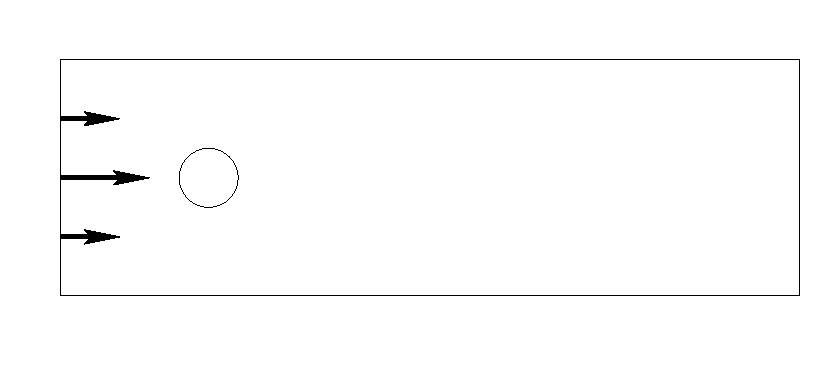
\includegraphics{Pictures/example_ns.pdf}%
\end{picture}%
\setlength{\unitlength}{4144sp}%
%
\begingroup\makeatletter\ifx\SetFigFontt\undefined%
\gdef\SetFigFontt#1#2#3#4#5{%
  \reset@font\fontsize{#1}{#2pt}%
  \fontfamily{#3}\fontseries{#4}\fontshape{#5}%
  \selectfont}%
\fi\endgroup%
\begin{picture}(6330,2785)(3136,-4652)
\put(9001,-4561){\makebox(0,0)[lb]{\smash{{\SetFigFontt{14}{16.8}{\familydefault}{\mddefault}{\updefault}{\color[rgb]{0,0,0}$(2.5,0)$}%
}}}}
\put(9001,-2086){\makebox(0,0)[lb]{\smash{{\SetFigFontt{14}{16.8}{\familydefault}{\mddefault}{\updefault}{\color[rgb]{0,0,0}$(2.5,0.41)$}%
}}}}
\put(3376,-2086){\makebox(0,0)[lb]{\smash{{\SetFigFontt{14}{16.8}{\familydefault}{\mddefault}{\updefault}{\color[rgb]{0,0,0}$(0,0.41)$}%
}}}}
\put(3376,-4561){\makebox(0,0)[lb]{\smash{{\SetFigFontt{14}{16.8}{\familydefault}{\mddefault}{\updefault}{\color[rgb]{0,0,0}$(0,0)$}%
}}}}
\put(7201,-3661){\makebox(0,0)[lb]{\smash{{\SetFigFontt{14}{16.8}{\familydefault}{\mddefault}{\updefault}{\color[rgb]{0,0,0}${\Omega}$}%
}}}}
\put(5851,-2086){\makebox(0,0)[lb]{\smash{{\SetFigFontt{14}{16.8}{\familydefault}{\mddefault}{\updefault}{\color[rgb]{0,0,0}$\Gamma_{wall}$}%
}}}}
\put(5851,-4561){\makebox(0,0)[lb]{\smash{{\SetFigFontt{14}{16.8}{\familydefault}{\mddefault}{\updefault}{\color[rgb]{0,0,0}$\Gamma_{wall}$}%
}}}}
\put(3151,-3211){\makebox(0,0)[lb]{\smash{{\SetFigFontt{14}{16.8}{\familydefault}{\mddefault}{\updefault}{\color[rgb]{0,0,0}$\Gamma_{in}$}%
}}}}
\put(9451,-3211){\makebox(0,0)[lb]{\smash{{\SetFigFontt{14}{16.8}{\familydefault}{\mddefault}{\updefault}{\color[rgb]{0,0,0}$\Gamma_{out}$}%
}}}}
\end{picture}%
}
\caption{Flow around a cylinder with 
circle-center $C=(0.2,0.2)$ and radius $r=0.05$.}
\label{fig:example_ns}
\end{figure}

We split the program into the parts \texttt{main.cc}, \texttt{functionals.h} and \texttt{localpde.h}. The \texttt{main.cc}-file is responsible for the declaration of various objects which have mostly to do with the \textit{discretization}, the \textit{solvers} and the general \textit{program sequence}, whereas the other two contain most of the problem-data -- especially the cell-wise contributions of the weak form, the right hand side and the functional. We give a brief explanation on every file in the following.

\subsubsection{\texttt{main.cc}}
In this file we gather the basic components that are necessary for the
solution process of a (stationary) partial differential equation. The
structure of the program is basically the same for every equation under
consideration, what changes is typically just the \textit{kind} of  finite
element or the linear solver. Here, a key issue is that we only need to pick 
some pre-implemented routines from the \dope{} library rather than 
implementing new features.


After the usual preamble, in which we include the necessary header-files from \deal{}, \dope{} and our own problem (i.e. \texttt{localfunctional.h} and \texttt{localpde.h}), we start by defining an instance of a \texttt{ParameterReader}-object, which handles run-time parameter.
\begin{lstlisting}
   ParameterReader pr;
\end{lstlisting}
In a text-file we might specify some problem-related parameters (for instance the viscosity $\nu$), but also general parameters for (non)-linear solvers and the output of computed data. 
After that, we create a triangulation of the domain $\Omega$ named \texttt{triangulation}.

Next, we create some quadrature rules (for the evaluation of integrals over
cells and faces) and a finite element appropriate for the PDE at hand. We
choose a Gaussian quadrature of a certain degree and the previously mentioned
Taylor-Hood element. These routines are quite standard in each finite element
software and we take advantage to take them from \deal{}.

Then, the two characteristic features \texttt{LocalPDE} and \texttt{LocalFunctional} objects come into play:
\begin{lstlisting}
  
  LocalPDE<VECTOR> local_pde;
  LocalFunctional<VECTOR> local_functional;

\end{lstlisting}
These hold the information of the PDE and the functional under consideration. Further explication is given below because
the definition of this classes is done separately in \texttt{localpde.h} resp.   \texttt{localfunctional.h}.

In the next step, we define an object of type \texttt{SpaceTimeHandler}, which handles all the things connected with the triangulation as well as the finite element space. This class is also capable of organizing degrees of freedom in time-dependent problems, hence the name. 
\begin{lstlisting}

  SpaceTimeHandler<TRIANGULATION, FE> dof_handler(triangulation,
                                                  finite_element);

\end{lstlisting}
There exist different versions of this class for forward as well as optimization problems. 

Now we have everything at hand to create an instantiation of type \texttt{PDEProblemContainer}. This basically represents the discretized problem, and bundles things like boundary conditions, the PDE, the functional and the discretization. First, we give the constructor the \texttt{local\_pde} and the \texttt{dof\_handler}.
\begin{lstlisting}

  PDEProblemContainer<LocalPDE> prob_container(local_pde,
                                               dof_handler);
\end{lstlisting}
After that, we add the functional under consideration and, because it is a boundary functional, we specify the part of the boundary on which the functional operates (this is done via a 'boundary color', $1$ represents $\Gamma_{circ}$).
\begin{lstlisting}

  prob_container.AddFunctional(&local_functional);
  prob_container.SetBoundaryFunctionalColors(1);

\end{lstlisting}
Next, we incorporate the Dirichlet data, which is given by the class \texttt{DirichleData}. Then we have to tell the \texttt{prob\_container} for which components and boundaries we prescribe the Dirichlet conditions. This is done via a boundary-color (0 stands for $\Gamma_D$) and a \texttt{std::vector<bool> comp\_mask = (true, true, false)}.
\begin{lstlisting}

  DirichletData dd;
  prob_container.SetDirichletBoundaryColors(0, comp_mask, dd);

\end{lstlisting}
Now we create the object which steers the whole solution process, the previously mentioned \texttt{StatPDEProblem}. It takes care of solving the discretized equation and evaluating the given functionals. The class depends actually on some template-parameters, so for the sake of abbreviation, we defined a typedef at the beginning of the \texttt{main.cc}-file.
\begin{lstlisting}

  typedef StatPDEProblem<NEWTONSOLVER,
           PDEProblemContainer<LocalPDE>, VECTOR, 2> SSOLVER;

\end{lstlisting}
Here, \texttt{NEWTONSOLVER} itself is an abbreviation of
\begin{lstlisting}
  
  typedef NewtonSolver<LINEARSOLVER, VECTOR, 2> NEWTONSOLVER;

\end{lstlisting}
The first template parameter of \texttt{NewtonSolver} describes which linear solver we use in this example. We opted for a direct solver, so: 
\begin{lstlisting}
  
  typedef DirectLinearSolverWithMatrix<MATRIX,
            VECTOR, 2> LINEARSOLVER;

\end{lstlisting}
With the type settled, we create the object \texttt{solver}, which needs the discretization (represented here by the \texttt{prob\_container}), the parameter reader as well as the quadrature rules.
\begin{lstlisting}

  SSOLVER solver(prob_container, pr,
                    quad_formula, face_quad_formula);

\end{lstlisting}
Finally, the program is started by
\begin{lstlisting}

  solver.ReInit();
  solver.ComputeReducedFunctionals();

\end{lstlisting}

\subsubsection{\texttt{localpde.h}}
We shall now give an overview to the implementation of the specific form of the PDE. 

Let $N$ be the number of degrees of freedom of our discretization and $\Set{\phi_{h}^{i}|1\leq i \leq N}$ be a given FE-Basis. As stated in subsection~\ref{subsubsec:stationary problems}, to solve the discrete equation \eqref{eq:discrete_equation} we need the residual, i.e. the vector
\begin{align}\label{eq:discrete_residual}
\left(a(u_h)(\phi_{h}^{i})-(f,\phi_{h}^{i})\right)_{i=1}^N,
\end{align}
and the Jacobi-matrix of the weak form, i.e.
\begin{align}\label{eq:discrete_matrix}
\left(\nabla a(u_h)(\phi_{h,j},\phi_{h}^{i})\right)_{i,j=1}^N.
\end{align}
Now all we have to supply here are the cell-wise contributions to these terms, the \texttt{Integrator} takes care of assembling \eqref{eq:discrete_residual} and \eqref{eq:discrete_matrix}.

To this end, we define a class \texttt{LocalPDE} which provides the three methods
\texttt{CellEquation}, \texttt{CellRightHandSide} and \texttt{CellMatrix}. The implementation of the terms works by and large as in \deal{}. We show the basic structure of these methods using the example of \texttt{CellEquation}.

\begin{lstlisting}
  void CellEquation(const CellDataContainer<2>& cdc,
                    VECTOR &local_cell_vector)
    {
      const auto& fe_values = cdc.GetFEValuesState();
      unsigned int n_dofs_per_cell = cdc.GetNDoFsPerCell();
      unsigned int n_q_points = cdc.GetNQPoints();
\end{lstlisting}
 The \texttt{CellDataContainer} contains all the information we need to compute the cell-contributions (things like number of quadrature points, number of degrees of freedom on the cell, the \texttt{dealii::FEValues}-objects, etc.).
  \begin{lstlisting}
     cdc.GetValuesState("last_newton_solution", uvalues);
     cdc.GetGradsState("last_newton_solution", ugrads);
 \end{lstlisting}
 In these two lines, we load the (gradient of the) solution of the last newton iteration in all the quadrature points on the cell into the two vectors \texttt{uvalues} and \texttt{ugrads}.

In the next lines, we finally implement our concrete PDE. Here, aim to provide 
an interface which is closely related to the weak formulation which 
has to be derived by the user. Thus,
we loop over the quadrature points and the number of DoFs of the cell. In the innermost loop, we evaluate the weak form tested with $\phi_{i,h}$ (represented by \texttt{phi\_i\_grads\_v}) on the cell with the help of the previously selected quadrature formula. 
 \begin{lstlisting}
    for(unsigned int q_point = 0; q_point < n_q_points; q_point++)
    {
      //initialize phi_i_grads_v etc.
      Tensor<2,2> vgrads;
      vgrads[0]= ugrads[q_point][0]; 
      vgrads[1]= ugrads[q_point][1];
      for (unsigned int i=0;i<n_dofs_per_cell;i++)
        local_cell_vector(i) += ( _nu 
                                * vgrads * phi_i_grads_v 
                                + //all the other terms)
                                * state_fe_values.JxW(q_point);
    }
\end{lstlisting}
\dope{} takes now care of the distribution of the local cell contributions into  the vector of the residual \eqref{eq:residual_vector}. The methods \texttt{CellRightHandSide} and \texttt{CellMatrix} follow the same structure as 
\texttt{CellEquation}, so we do not go into the details here.

\subsubsection{\texttt{localfunctional.h}}
The implementation of the boundary-functional $J$ follows the outline of the computation of the cell-residual in \texttt{localpde.h}. However, there are two main differences. First, we do not have to specify the method \texttt{CellEquation}, but \texttt{BoundaryValue} instead. This is due to the fact that we consider a boundary-functional in this example, and so we have to specify the value of the functional not cell-wise but face wise (for the faces that lie on $\Gamma_{circ}$). The second difference is that as we only want to evaluate a functional and not a residual-vector, we just loop over the quadrature points and not over the degrees of freedom on the face.
\begin{lstlisting}
 double
 BoundaryValue(const FaceDataContainer<2>& fdc)
  {
    //same as before, get n_q_points etc.
    fdc.GetFaceValuesState("state", ufacevalues);
    fdc.GetFaceGradsState("state", ufacegrads);
\end{lstlisting}
Notice that we get here the values of the computed solution by giving the string "state".
\begin{lstlisting}
    for(unsigned int q_point = 0; q_point < n_q_points; q_point++)
      erg += -1. * ( _nu * ufacegrads[q_point][0]
                * state_fe_face_values.normal_vector(q_point)
                + //other terms)        
                * state_fe_face_values.JxW(q_point);
    return erg;
  }
\end{lstlisting}

\subsection{Solving Nonstationary PDEs}\label{sec:timedep}
To describe the solution of nonstationary 
PDEs, we consider a time-dependent semi-linear form $a(u)(\phi)$ and some
right hand side functional $l(\phi)$.
Let $I:=[0,T]$ be a time interval with end time point value $T$.
To find some $u$ in a weak form, we define
\[
\int_I a(u)(\phi)\, dt = \int_I l(\phi)\, dt \quad \forall\Phi\in X,
\]
with some suitable Bochner space $X$.  As model problem,
we consider the nonstationary Navier-Stokes equations
in a domain $\Omega\in\mathbb{R}^d$. Find: 
$(v,p)\in X$ with
\[
\int_I \bigl[ (\partial_t v, \phi)
+ \nu (\nabla v, \nabla \phi) + (v\cdot\nabla v, \phi)
- (p,\nabla\cdot \phi)
+ (\nabla\cdot v, \chi)\bigr] \, dt
+ (v(0) - v^0, \phi(0))
= \int_I l(\phi) \, dt 
\]
for all $\Phi:= (\phi, \chi) \in X$ with
\[
X:= \bigl\{ 
(v,p) | v\in L^2(I,H_0^1(\Omega)^d) , 
\partial_t v\in L^2(I, L^2(\Omega)^d), 
p\in L^2(I,L^2(\Omega)\setminus\mathbb{R} \bigr\}.
\]
As for stationary problems, the goal is to compute
some target functional $J(\cdot)$ which is now possibly 
time-dependent. To organize the discretization 
process, we need to perform spatial and temporal 
discretization. This is again done via
an object that takes care of organizing the degrees of 
freedom, as in the case of stationary problems.
The only difference to the stationary case is that we need to 
add the temporal subdivision \texttt{times}. In the simplest 
case, when we have the same spatial triangulation 
at all times, the constructor could look as follows:
\begin{lstlisting}
  template<typename Triangulation, typename FE, typename times>
      void SpaceTimeHandler(Triangulation &, FE, times&);
\end{lstlisting}

Now we may discretize the problem with some time-stepping scheme, which will 
remove the temporal derivative and replace it by some difference quotients. 
Since the exact way of doing this depends on the time-stepping scheme 
we need a new object that takes the user-given description of the PDE and 
generates the appropriate combinations of spatial integrals and scaling.
Thus a generic problem may look as follows:
\begin{lstlisting}
  template<typename PROBLEM>
      class TimeStepProblem;
\end{lstlisting}
At present we have prepared the following time-stepping schemes in \dope:
\begin{itemize}
\item Forward-(Explicit)-Euler
\item Backward-(Implicit)-Euler
\item Crank-Nicolson scheme
\item shifted Crank-Nicolson scheme (to deal with singular initial data)
\item fractional-step-$\theta$ scheme
\end{itemize}
With this we can now run a loop over all time-steps, where in each of the 
time-steps we can reuse the functionality to solve stationary PDEs 
applied to the time-step problem. 

Now it is apparent, why we introduced the \texttt{StatPDEProblem}, because
we now define the \texttt{InstatPDEProblem} to contain the necessary 
loop over all time points. Next, we will describe the methods the user needs to 
provide in addition to the stationary case.

\subsubsection{Problem-dependent 
implementation of nonstationary problems}
\label{sec:timedep:implementation}
We explain in more detail the temporal discretization
and specific issues of its implementation. 
To keep the presentation easy, we abuse notation 
by neglecting
all material coefficients
and give formal-related idea based on the weak 
form of the Navier-Stokes equations:
Find $(v,p)$ such that
\begin{align*}
(\partial_t v,\phi) 
+ (\nabla v, \nabla \phi)
+ (v\cdot\nabla v,\phi)
-(p,\nabla\cdot \phi)
+(\nabla\cdot v, \chi)
=(f,\phi),
\end{align*}
where $f$ describes some volume forces.
Temporal discretization using the One-step-$\theta$ scheme reads:
Given the old time-step solution $(v^n,p^n)$, 
find $(v^{n+1}, p^{n+1})$ (and multiplication 
by the inverse of the time-step $k$):
\begin{align*}
(v^{n+1} - v^{n}, \phi)
&+ k\theta (\nabla v^{n+1}, \nabla \phi)
+ k\theta (v^{n+1}\cdot\nabla v^n + 
  v^{n}\cdot\nabla v^{n+1},\phi)\\
&- k (p^{n+1},\nabla\cdot \phi)
+ (\nabla\cdot v^{n+1}, \chi)\\
=&\; k\theta (f^{n+1},\phi) + k(1-\theta) (f^{n},\phi)
- k(1-\theta) (\nabla v^{n}, \nabla \phi) 
\end{align*}
The concrete choice of $\theta$ leads to a
specific time-stepping scheme. For instance,
$\theta = 0.5$ gives the Crank-Nicolson scheme,
\begin{lstlisting}
   CrankNicolsonProblem<...>
\end{lstlisting}


The pressure and incompressibility terms should be 
treated fully implicitly when time-discretizing 
the Navier-Stokes equations.
For this reason, the implementation is split up
into several items to account for fully implicit 
terms and remaining terms for which we need 
old time-step and present time-step values. 
Hence, in the local cell equation, the parameters
\texttt{scale} and \texttt{$scale_ico$}
are used to distinguish these terms:
\begin{lstlisting}
  void CellEquation(...)
   {
      local_cell_vector(i) +=  
          scale * (\nabla v^{n+1}, \nabla \phi) + etc.

      local_cell_vector(i) +=  
          scale_ico * (-p^{n+1},\nabla\cdot v)
   }
\end{lstlisting}
Analogous procedure is performed in the local 
cell matrix.

In addition to stationary problems, the implementation
of the time-derivative must be considered which is done
in 
\begin{lstlisting}
  void CellTimeEquation(...)
   {
     local_cell_vector(i) += 
         scale * (u^{n+1},\phi) + etc. 
   }
\end{lstlisting}
and it is done in a straight-forward way:
\begin{lstlisting}
  for (all quadrature points per cell q)
   {
     Tensor<1,2> u = ...;

     for (all dofs per cell i)
      {
        const Tensor<1,2> phi_i_u = ...;

        local_cell_vector(i) +=  
          scale * (u * phi_i_u) * 
          state_fe_values.JxW(q_point);
      }
   }
\end{lstlisting}
Here, the advantage is that \dope{} orders the terms in the time-stepping
problems
such that only $(u^{n+1},\phi)$ must be implemented. 



\begin{remark}[Nonlinear terms in the time derivative]
However, if someone 
needs explicit input of the old time-step term, then he can use 
\begin{lstlisting}
  void CellTimeEquationExplicit (...)
   {
     // implement (u^{n+1},\phi) and (u^n,\phi)  
   }
\end{lstlisting}
\end{remark}

\begin{remark}[Fractional-Step-$\theta$-scheme]
The temporal discretization in this section 
is based on the One-Step-$\theta$-schemes. The library
offers in addition an implementation 
of the second-order and strongly $A$-stable 
Fractional-Step-$\theta$-scheme in which 
each time-step is subdivided into three 
sub-steps. 
\end{remark}

\subsection{Solving of optimization problems}\label{sec:opt}
Upgrading the framework for solving optimization problems
is described in this section. A prototypical problem reads:
\begin{align*}
\min\;&J(q,u) \\
  &\text{s.t.}\; a(q,u)(\phi) = 0 \quad \forall \phi\in V,\\
  &a \le q \le b,\\
  &g(q,u) \le 0,  
\end{align*}
where $u$ is a FE-function and $q$ can either be a FE-function or some 
fixed number of parameters, $a$ and $b$ are constraint bounds for the control $q$,
and $g(\cdot)$ is some state constraint.
To keep the presentation brief we will neglect the additional bounds
\[
a \le q \le b,\qquad g(q,u) \le 0
\]
although they can be treated by \dope{} as well.
Then, in order to minimize the functional $J$ one may apply the, so-called, 
reduced approach, in which we eliminate the dependent variable $u$ by the solution 
operator $S$ of the PDE, i.e., 
\begin{align*}
a(q,S(q))(\phi) = 0 \quad \forall \phi\in V. 
\end{align*}
This leads to the problem
\begin{align*}
\min\;&j(q) = J(q,S(q)). 
\end{align*}
Then, one can apply any algorithm to solve the, unconstraint, minimization 
problem. This, will in any case require the evaluation of $j(q)$ which 
we can do, e.g., using \texttt{StatPDEProblem::ComputeReducedFunctional} for 
a stationary PDE. If one would like to use derivative based methods, one 
needs in addition derivatives of $j$ and thus of $J$ as well as of $S$. 
To do so, we remark, that one can calculate the derivative of 
$j$ using the adjoint calculus. Then the directional derivative 
of $j$ in direction $\delta q$ is given by
\[
j'(q)(\delta q) = J'_q(q,S(q))(\delta q) + (S^* J_u'(q,S(q)),\delta q)
\]
where the index $q$ or $u$ denote directional derivatives for the 
respective argument. To calculate action of the adjoint operator $S^*$ 
we note that $z =  S^* J_u'(q,S(q))$
can be computed via the adjoint PDE
\begin{equation}
  \label{opt_KKT_system}
  \begin{aligned}
    a_{u}'(q,u)(\phi , z) &= J'_{u}(q,u)(\phi) & \forall \phi&\in {\cal X}.
  \end{aligned}
\end{equation}
Similarly formulas for the second derivatives can be obtained.

To do so, we define an object 
\begin{lstlisting} 
  template<typename PDE, typename COSTFUNCTIONAL>
    class OPTProblemContainer;
\end{lstlisting}
that collects the user given PDE and functional descriptions and constructs the 
required PDE and right hand side information needed for the calculations.

This means for the user only the derivatives of the functional and the PDE 
needs to be provided in addition to the 
\begin{lstlisting} 
  void CellEquation_U(...)
   {
     // implement directional derivative of the CellEquation
   }
\end{lstlisting}
and functional terms, i.e.,     
\begin{lstlisting} 
  virtual void BoundaryValue_U(...)
      {
        // implement here the derivative of 
        // the boundary cost functional
      }
\end{lstlisting}

Due to the design of the classes it is easily possible to extend any given 
and running code for a PDE both to the nonstationary counterpart, if the PDE is 
stationary, as well as to an optimization problem where the constraint is 
given by this PDE. Meaning that the use of our framework for the simulation of 
PDEs will, due to the enforced interface, enable easy application of state-of-the-art 
optimization algorithms to minimization problems governed by the PDE.


\subsection{Additional features}
Finally, we shall give a brief summary of features 
that are applicable (in general) to all types of problems. Specifically,
\dope{} provides goal-oriented mesh refinement with the help of the 
Dual Weighted Residual (DWR) method, see \cite{BeRa96} or \cite{BR03}. Here, a certain 
cost functional such as a point evaluation, line integration or domain
integration is considered. Determining the lowest error between the 
(unknown) exact solution and its numerical approximation for lowest computational
cost is the main goal of the DWR method. The same routines 
can also be used, without any modification, to use standard residual error estimators by exchanging the 
error estimator class.

Since in many applications it is desirable to use different discretizations
for the state and the control \dope{} provides multi-mesh support, meaning that
once a problem has been written correctly using the same mesh for all finite element
variables one can switch to a different SpaceTimeHandler that allows different meshes for all 
variables without the need to change the user-given implementation of the PDE and functional.

%%%%%%%%%%%%%%%%%%%%%%%%%%%%%%%%%%%%%%%%%%%
\section{Applications}
\label{applications}
In this final section, 
we present three numerical tests which demonstrate different
features of \dope{}:
\begin{itemize}
\item In the first numerical example, we consider 
goal-oriented mesh refinement with the help of the 
DWR method for the stationary Navier-Stokes equations.
\item The second example presents nonstationary fluid-structure 
interaction. The challenges for those kind of problems are the multi-domain
character of the coupled problem and the treatment of the coupling conditions.
The problem is formulated in a variational monolithically-coupled way which 
allows to consider goal-oriented mesh refinement and gradient-based optimization.
\item In the third numerical test, an optimization problem for structural mechanics
is discussed.
\end{itemize}

\subsection{Goal-oriented mesh refinement for Navier-Stokes}
In this example we consider a laminar flow around a cylinder in 2d. To be more precise, we are computing the benchmark 2D-1 from \cite{TuSchae96}. The computational domain is as depicted in figure~\ref{fig:example_ns}. We want to compute the drag force on the enclosed cylinder
\begin{equation}
c_D = \frac 1 {20} \int_{\Gamma_{circ}} \nu\partial_nu _1 - pn,
\end{equation}
with the normal $n$ and $\nu = 0.001$. To achieve an efficient computation of the quantity $c_D$, we employ goal-oriented mesh refinement with the help of the DWR-method, see \cite{BeRa96}.

\begin{itemize}
\item Bild Freiheitsgrade vs Fehler, global und 
\item Bild adaptive mesh, bild der Loesung (?)
\item eventuell kurz auf duale gleichung eingehen.
\end{itemize}

\subsection{Nonstationary Fluid-Structure Interaction}
In this example, a challenging benchmark FSI 2
proposed by Hron and Turek \cite{HrTu06b} is considered.
To solve this problem accurately, it is very important that 
the coupling conditions
\[
v_f = v_s \quad \text{and} \quad \sigma_f n_f = \sigma_s n_s, 
\]
namely, the continuity of velocities and continuity of normal stresses
are satisfied in each time-step. This is achieved with the help of 
a monolithic coupling scheme (strong coupling).

The basic configuration is 
sketched in Figure \ref{fig:example_ns} at which an elastic beam is attached 
behind the rigid cylinder. 
The computational domain has length $L=2.5m$ and height $H=0.41m$. The circle center
is positioned at $C=(0.2m,0.2m)$ with radius $r=0.05m$. The elastic beam has length
$l=0.35m$ and height $h=0.02m$. The right lower end is positioned at 
$(0.6m,0.19m)$, and
the left end is attached to the circle. 
Control points $A(t)$ (with $A(0) = (0.6,0.2)$) are fixed at the 
trailing edge of the structure, measuring $x$- and $y$-deflections of the beam.

Details 
on parameters and evaluation functionals and other results 
can be found in \cite{HrTu06b,BuSc06,DeHaeAnnBrVie10,Wi11}. 
The Fractional-Step-$\theta$ scheme is used for time discretization with
different time step sizes $k$. However, the time-stepping scheme can be 
very easily chosen in the \texttt{main.cc} function by choosing an appropriate 
time-stepping scheme, at present the following are available.
\begin{lstlisting}
ForwardEulerProblem
BackwardEulerProblem
CrankNicolsonProblem
ShiftedCrankNicolsonProblem
FractionalStepThetaProblem
\end{lstlisting}

The quantities of interest are evaluations of 
$x$- and $y$ displacement at the point $A(0) = (0.6,0.2)$
and the drag and lift forces acting on the cylinder and the elastic beam:
\begin{align}
\label{drag_lift_forces}
(F_D , F_L) 
= {\int_{S_f} \sigma_f \cdot n_f \, ds + 
\int_{\Gamma_i} \sigma_s \cdot n_s \, ds},
\end{align}
where $S_{f}$ denotes the path over the cylinder in the fluid part and
$\Gamma_i$ the interface between the elastic beam and the 
fluid.

Since the problem is fully nonstationary, the 
dynamics are presents in Figure \ref{res:fsi_2_mesh_and_x_velo}. 
By comparison of our findings in Figure \ref{res:results_ux_and_uy_fsi_2}
with the literature, it can be identified that 
the implementation in \dope{} is correct.



% Bilder von FSI 2 
\begin{figure}[h]
\centering
{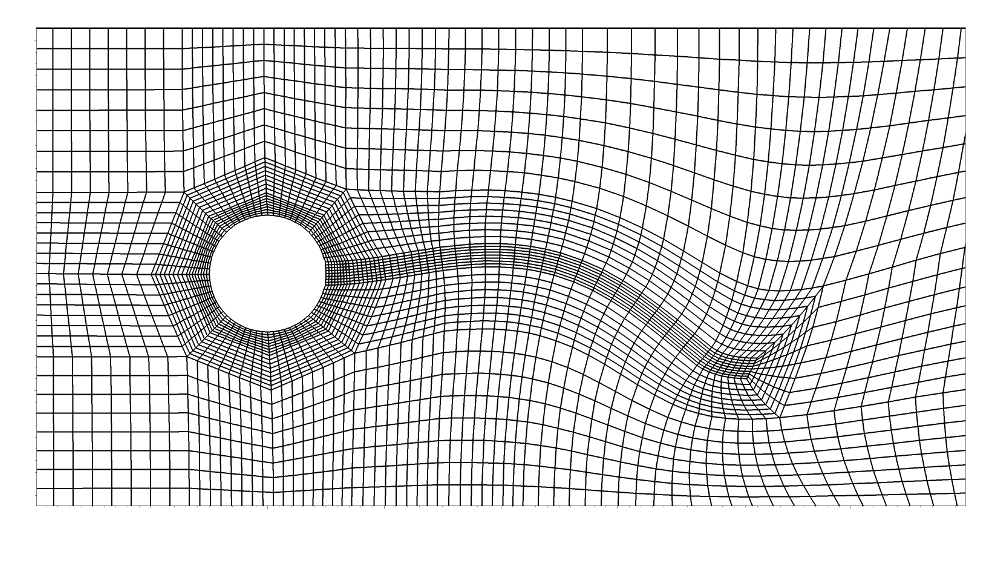
\includegraphics[width=6cm]{Pictures/visit_fsi_2_CNn_t_2e-2_global_3_biharmonic_mesh8070_scale.png}}
{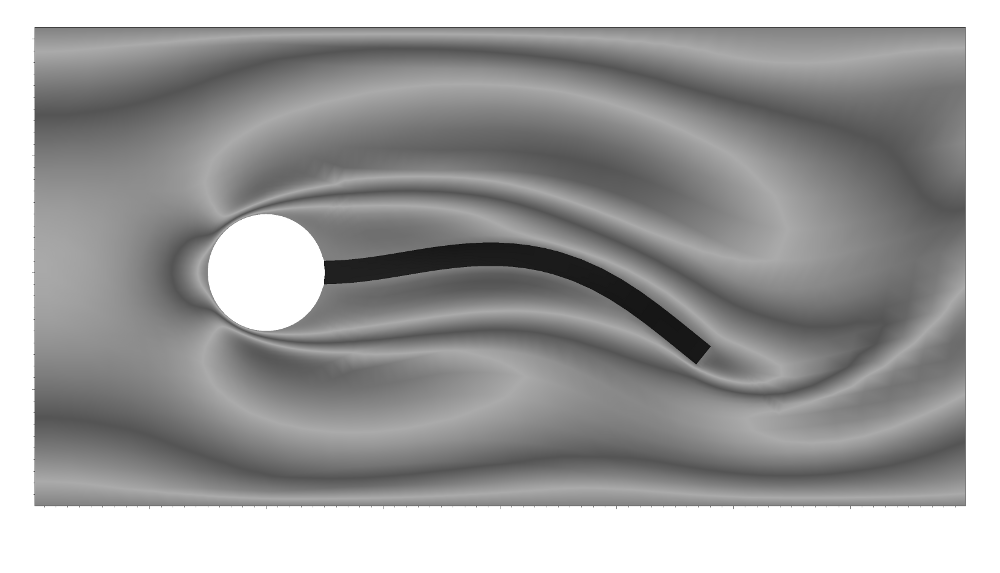
\includegraphics[width=6cm]{Pictures/visit_fsi_2_CNn_t_2e-2_global_3_biharmonic_x_velo8070_scale.png}}
\caption{FSI 2 test case: mesh (left) and velocity profile in vertical 
direction (right) at time $t=16.14s$.}
\label{res:fsi_2_mesh_and_x_velo}
\end{figure}

\begin{figure}
\centering
{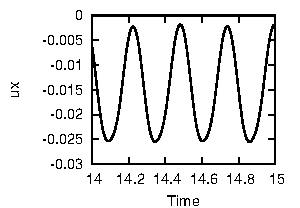
\includegraphics[width=5.8cm]{Pictures/ux_FSI_2_FS_t_3e-2_t_15e-3_global_2_Hron_grid.pdf}}
{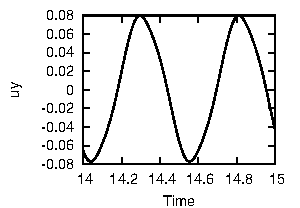
\includegraphics[width=5.8cm]{Pictures/uy_FSI_2_FS_t_3e-2_t_15e-3_global_2_Hron_grid.pdf}}
{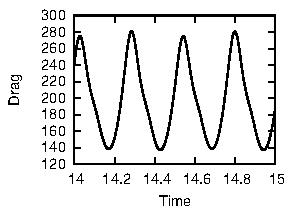
\includegraphics[width=5.8cm]{Pictures/Drag_fluid_FSI_2_FS_t_3e-2_t_15e-3_global_2_Hron_grid.pdf}}
{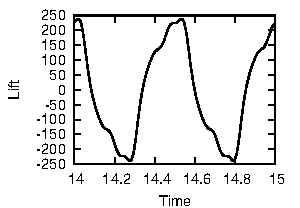
\includegraphics[width=5.8cm]{Pictures/Lift_fluid_FSI_2_FS_t_3e-2_t_15e-3_global_2_Hron_grid.pdf}}
\caption{FSI 2: the deflections of the beam, $u_x(A)$ and $u_y(A)$ (in $cm$), and 
the drag $F_D$ and the lift $F_L$ evaluation (in $kg/m\,s^2$) are displayed versus
time (in $s$).
} 
\label{res:results_ux_and_uy_fsi_2}
\end{figure}


\newpage
\subsection{Compliance minimization}
In this example, we consider the compliance minimization of a standard MBB-Beam. 
The thickness variable is allowed to take intermediate value apart from $0$ and $1$,
i.e., we consider a variable thickness sheet. The discretization is done 
using $Q_2$ elements for the displacement and discontinuous $P_0$ elements for the 
thickness.
\begin{figure}
\centering
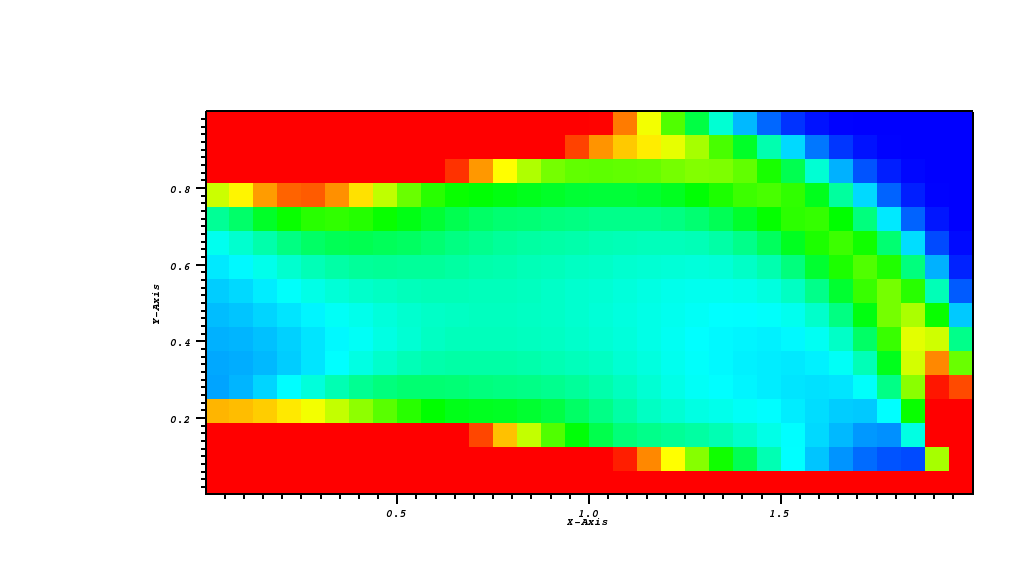
\includegraphics[width=1.\textwidth, viewport=150 0 1024 500, clip]{Pictures/MBB.png}
\caption{Thickness distribution for the MBB-beam minimum compliance problem.} 
\label{res:mbb}
\end{figure}
A typical thickness distribution is shown in Figure~\ref{res:mbb}.


\section*{Thanks}
The \dope{} project makes use of various finite elements taken from  
the \deal{} \cite{dealnew} finite element library which has been developed
 initially by W. Bangerth, R. Hartmann, and G. Kanschat \cite{dealold}.
The authors acknowledge their past experience as well as discussions 
on modularization of algorithms
with 
the authors of the libraries 
Gascoigne/RoDoBo project, which was initiated by 
Roland Becker, Dominik Meidner, and Boris Vexler \cite{rodobo}. 
The second author thanks Mary F. Wheeler (ICES, Austin) for the 
possibility to finish this work.

%%%%%%%%%%%%%%%%%%%%%%%%%%%%%%%%%%%%%%%%%%%
%\bibliographystyle{abbrvnat}
\bibliographystyle{acmsmall}
\bibliography{lit}
%


\end{document}


